\documentclass[tikz,border=3pt]{standalone}
% Shared preamble for the v2 figures.
% Fonts: acmart's pdfLaTeX set (Libertine text, newtxmath[libertine]) when
% installed; otherwise Latin Modern. Recompile once Libertine is installed.
\usepackage[T1]{fontenc}
\usepackage{amsmath}
\IfFileExists{libertine.sty}{%
  \IfFileExists{newtxmath.sty}{%
    \usepackage[tt=false,type1=true]{libertine}%
    \usepackage[libertine]{newtxmath}%
  }{\usepackage{lmodern}}%
}{\usepackage{lmodern}}
% Colours: Okabe--Ito-derived, distinguishable in greyscale by luminance
% and always paired with a second cue (line weight, dash, marker shape).
\definecolor{editblue}{HTML}{193E57}  % dark: paths, peeling steps, branch
\definecolor{lawgray}{HTML}{81888C}   % mid grey: constraint sets, context
\definecolor{pointver}{HTML}{D55E00}  % vermillion: forced points, blocks
\newcommand{\lab}[1]{\mathsf{#1}}     % labels in sans serif

\usepackage{pgfplots}
\pgfplotsset{compat=1.18}
\usetikzlibrary{arrows.meta,shapes.geometric}


\begin{document}
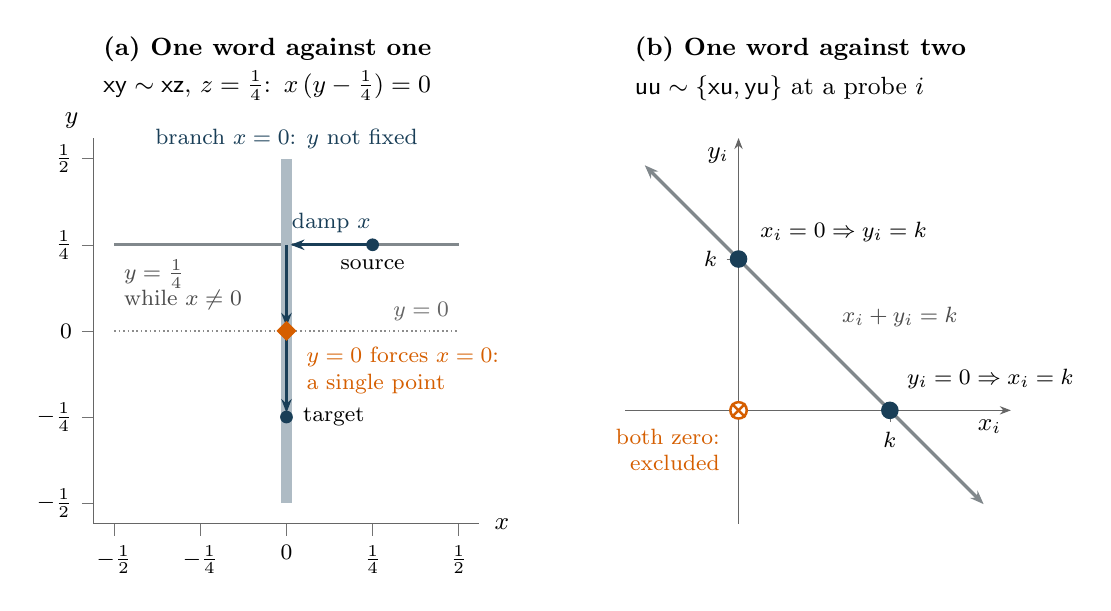
\begin{tikzpicture}[
  every node/.style={font=\small},
  pathstep/.style={editblue,line width=1.1pt,-{Stealth[length=5pt]}},
]
%-------------------------------------------------------------- panel (a)
\begin{axis}[
  name=pa,
  width=4.9cm, height=4.9cm, scale only axis,
  xmin=-0.56, xmax=0.56, ymin=-0.56, ymax=0.56,
  axis lines=left, axis line style={-, black!60},
  tick align=outside, tick style={black!55},
  ticklabel style={font=\footnotesize},
  xtick={-0.5,-0.25,0,0.25,0.5}, ytick={-0.5,-0.25,0,0.25,0.5},
  xticklabels={$-\frac12$,$-\frac14$,$0$,$\frac14$,$\frac12$},
  yticklabels={$-\frac12$,$-\frac14$,$0$,$\frac14$,$\frac12$},
  xlabel={$x$}, ylabel={$y$},
  xlabel style={at={(axis description cs:1,0)},anchor=west,xshift=2pt},
  ylabel style={at={(axis description cs:0,1)},anchor=south east,rotate=-90,xshift=-2pt},
  clip=false,
]
% the line y = 0 (dotted), meeting the feasible cross only at the origin
\addplot[black!45, densely dotted, line width=0.6pt] coordinates {(-0.5,0) (0.5,0)};
\node[font=\footnotesize, text=black!60, anchor=south east] at (axis cs:0.5,0) {$y=0$};
% feasible cross: y = 1/4 with |x| <= 1/2 (thin grey) ...
\addplot[lawgray, line width=1.2pt] coordinates {(-0.5,0.25) (0.5,0.25)};
\node[font=\footnotesize, text=black!70, anchor=north west, align=left] at (axis cs:-0.5,0.235) {$y=\frac14$\\while $x\neq0$};
% ... and the branch x = 0 with |y| <= 1/2 (thick, dark)
\addplot[editblue!35, line width=4.2pt] coordinates {(0,-0.5) (0,0.5)};
\node[font=\footnotesize, text=editblue, anchor=south, align=center] at (axis cs:0,0.5)
  {branch $x=0$: $y$ not fixed};
% staged revision (1/4,1/4) -> (0,1/4) -> (0,0) -> (0,-1/4)
\draw[pathstep] (axis cs:0.25,0.25) -- (axis cs:0.012,0.25);
\draw[pathstep] (axis cs:0,0.25) -- (axis cs:0,0.012);
\draw[pathstep] (axis cs:0,0) -- (axis cs:0,-0.238);
% endpoints
\fill[editblue] (axis cs:0.25,0.25) circle (2.3pt);
\fill[editblue] (axis cs:0,-0.25) circle (2.3pt);
\node[anchor=north, font=\footnotesize] at (axis cs:0.25,0.235) {source};
\node[anchor=west, font=\footnotesize] at (axis cs:0.02,-0.25) {target};
\node[anchor=south, font=\footnotesize, text=editblue] at (axis cs:0.13,0.255) {damp $x$};
% the point forced by y = 0
\node[draw=pointver, fill=pointver, diamond, inner sep=1.7pt] at (axis cs:0,0) {};
\node[anchor=north west, font=\footnotesize, text=pointver, align=left]
  at (axis cs:0.03,-0.02) {$y=0$ forces $x=0$:\\a single point};
\end{axis}
\node[anchor=south west, font=\small\bfseries] at ([yshift=24pt]pa.north west)
  {(a) One word against one};
\node[anchor=south west, font=\small] at ([yshift=10pt]pa.north west)
  {$\lab{x}\lab{y}\sim\lab{x}\lab{z}$, $z=\tfrac14$:\enspace $x\,(y-\tfrac14)=0$};

%-------------------------------------------------------------- panel (b)
\begin{axis}[
  name=pb, at={(6.75cm,0)},
  width=4.9cm, height=4.9cm, scale only axis,
  xmin=-0.75, xmax=1.8, ymin=-0.75, ymax=1.8,
  axis lines=middle, axis line style={-{Stealth[length=4pt]}, black!60},
  tick align=outside, tick style={black!55},
  ticklabel style={font=\footnotesize},
  xtick={1}, ytick={1}, xticklabels={$k$}, yticklabels={$k$},
  xlabel={$x_i$}, ylabel={$y_i$},
  xlabel style={anchor=north east}, ylabel style={anchor=north east},
  clip=false,
]
% the zero set of the load equation x_i + y_i = k, past both axes
\draw[lawgray, line width=1.2pt, {Stealth[length=5pt]}-{Stealth[length=5pt]}]
  (axis cs:-0.62,1.62) -- (axis cs:1.62,-0.62);
\node[font=\footnotesize, text=black!70, anchor=west]
  at (axis cs:0.62,0.62) {$x_i+y_i=k$};
% axis points (k,0) and (0,k)
\node[draw=editblue, fill=editblue, circle, inner sep=2.1pt] at (axis cs:1,0) {};
\node[draw=editblue, fill=editblue, circle, inner sep=2.1pt] at (axis cs:0,1) {};
\node[font=\footnotesize, anchor=south west, align=left] at (axis cs:1.05,0.08)
  {$y_i=0\Rightarrow x_i=k$};
\node[font=\footnotesize, anchor=south west, align=left] at (axis cs:0.08,1.05)
  {$x_i=0\Rightarrow y_i=k$};
% origin excluded
\node[draw=pointver, fill=white, circle, inner sep=2.1pt, line width=0.9pt] at (axis cs:0,0) {};
\draw[pointver, line width=0.9pt] (axis cs:-0.045,-0.045) -- (axis cs:0.045,0.045)
  (axis cs:-0.045,0.045) -- (axis cs:0.045,-0.045);
\node[font=\footnotesize, text=pointver, anchor=north east, align=right]
  at (axis cs:-0.06,-0.06) {both zero:\\excluded};
\end{axis}
\node[anchor=south west, font=\small\bfseries] at ([yshift=24pt]pb.north west)
  {(b) One word against two};
\node[anchor=south west, font=\small] at ([yshift=10pt]pb.north west)
  {$\lab{u}\lab{u}\sim\{\lab{x}\lab{u},\lab{y}\lab{u}\}$ at a probe $i$};
\end{tikzpicture}
\end{document}
